\begin{sol}
\begin{enumerate}[label=\textbf{(\alph*)}]
\item The differential equation we get is:
$$(E_x+E_y)\Psi=-\frac{\hbar^2}{2m}\left(\frac{\partial^2}{\partial x^2}+\frac{\partial^2}{\partial y^2}\right)\Psi$$
We can break this up into the $x$ and $y$ solutions, and then multiply them together to get:
$$\Psi = \frac{2}{\sqrt{L_xL_y}}\sin\left(\frac{n_x \pi x}{L_x}\right)\sin\left(\frac{n_y \pi y}{L_y}\right)$$
such that the energy eigenstates are
$$E=\frac{\hbar^2\pi^2n_x^2}{2mL_x^2}+\frac{\hbar^2\pi^2n_y^2}{2mL_y^2}$$
\item If $L_x=L_y=L$, we get:
$$E=\frac{\hbar^2\pi^2}{2mL^2}(n_x^2+n_y^2)$$
and if $n_x$ and $n_y$ are plotted, they trace out a parabaloid. Given a particular circular cross section, all points on the circumference with integer coordinates represent degenerate energies. 
\begin{center}
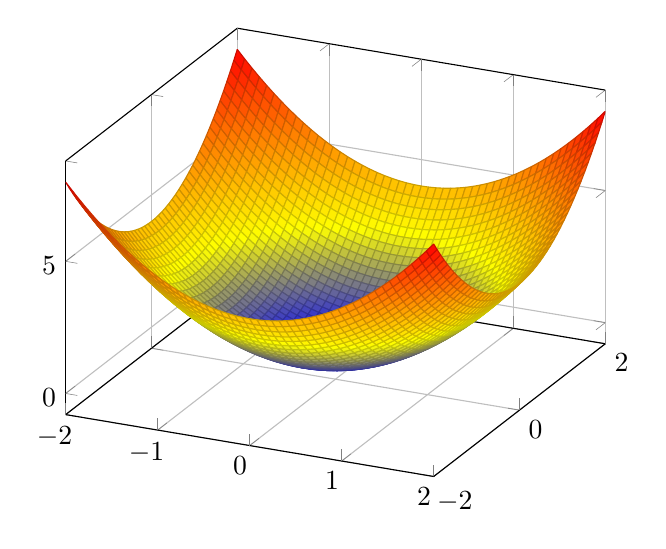
\begin{tikzpicture}
  \begin{axis}[grid=both,restrict z to domain*=0:10]
    \addplot3 [surf,samples=51,
        domain=-2:2,miter limit=1] {x^2 + y^2};
  \end{axis}
\end{tikzpicture}
\end{center}
This is now essentially a number theory problem involving diophantine equations. While a pattern can emerge by repeatedly applying the Brahmagupta–Fibonacci identity, these do not really hold any physical insight. For example:
$$(n_x,n_y)=(33,56)$$
gives the same energy as
$$(n_x,n_y)=(63,16).$$
However, there are also degenerate energies that are not coincidences. For example, if the ordered pair $(n_x,n_y)$ gives a certain energy, then $(n_y,n_x)$ also gives the same energy. This can be interpreted as a rotation of the wavefunction, meaning that if the $x$ and $y$ components are swapped, it would make no difference.
\item This in a sense, is mainly a number theory problem. We want to show that:
$$\frac{n_x^2}{L_x^2}+\frac{n_y^2}{L_y^2}=\frac{n_x'^2}{L_x^2}+\frac{n_y'^2}{L_y^2}$$
has no nontrivial integers solutions given that $(L_x/L_y)^2$ is irrational. We will do this via contradiction. Suppose $k\equiv (L_x/L_y)^2$ is irrational and there are integer solutions (which represent degeneracies), then:
$$n_x^2+kn_y^2=n_x'^2+kn_y'^2 \implies k=\frac{n_x^2-n_x'^2}{n_y'^2-n_y^2}$$
Since $n$ is an integer, then the numerator and denominators must also be integers, and thus $k$ is rational, contradicting our claim.
\end{enumerate}
\end{sol}